%%This is a very basic article template.
%%There is just one section and two subsections.
\documentclass[12pt, twoside]{article}
\usepackage[francais]{babel}
\usepackage[T1]{fontenc}
\usepackage[latin1]{inputenc}
\usepackage[left=7mm, right=1cm, top=1cm, bottom=7mm]{geometry}
\usepackage{float}
\usepackage{graphicx}
\usepackage{array}
\usepackage{multirow}
\usepackage{amsmath,amssymb,mathrsfs}
\usepackage{soul}
\usepackage{textcomp}
\usepackage{eurosym}
 \usepackage{variations}
\usepackage{tabvar}

\begin{document}
\ul{Exercice 10:}
\begin{center}
	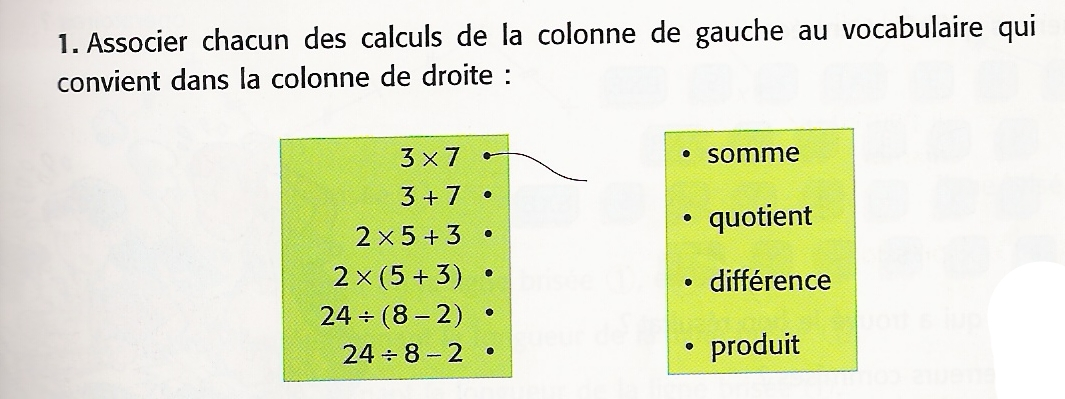
\includegraphics[width=11cm]{images/exo10.jpg}
\end{center}

\bigskip

\ul{Exercice 11:}


\begin{enumerate}
	\item Traduire par un calcul les phrases suivantes : 
		\begin{enumerate}
		  \item Le produit de 4 par la somme de 7 et de 8.
		  \item La somme de 6 et du produit de 9 par 4.
		  \item La diff�rence de 68 et du quotient de 24 par 3.
		  \item Le produit de 7 par la diff�rence de 15 et 9.
		\end{enumerate}
	\item Effectuer les calculs.
\end{enumerate}

\bigskip

\ul{Exercice 12:}


\begin{center}
	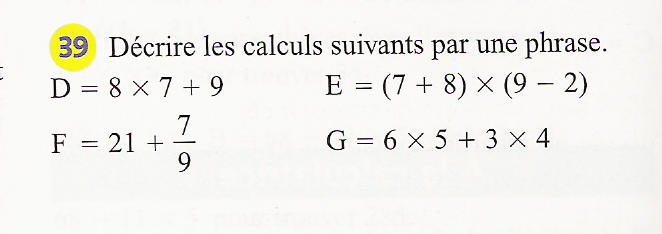
\includegraphics[width=8cm]{images/exo12.jpg}
\end{center}

\bigskip

\ul{Exercice 13:} Soit $A=4n$ et $B=4+n$.

\begin{enumerate}
  \item R��crire l'expression $A$ en faisant appara�tre le signe ``$\times$''
  qui a �t� supprim�.
  \item Calculer $A$ et $B$ pour les valeurs suivantes de $n$:
  
  \begin{enumerate}
    \item $n=8$
    \item $n=11$
    \item $n=0$
    \item $n=1,2$
\end{enumerate}

\end{enumerate}

\bigskip

\ul{Exercice 14:} Calculer $3a+5b$ dans les cas suivants:

\begin{enumerate}
  \item $a=8$ et $b=6$
  \item $a=6$ et $b=8$
\end{enumerate}
\end{document}
